\section{Les NN}

\begin{frame}
 \frametitle{Sélection d'un réseau de neurones}
 Réseaux de neurones qui seront présentés:\\
 \begin{itemize}
  \item Les \emph{feedforwards}, c'est-à-dire \textbf{non récurrents}:\\
   \begin{itemize}
    \item \alert{\emph{Perceptron multi-couches}} (MLP)
    \item \alert{\emph{Fonction à base radiale}} (RBF) %TODO verifier
   \end{itemize}
  \item Les \textbf{récurrents}:\\
   \begin{itemize}
    \item \alert{\emph{Perceptron multi-couches récurrent}} (RMLP)
   \end{itemize}
 \end{itemize}
\end{frame}

\subsection{Perceptron multi-couches}
\begin{frame}
 \frametitle{Perceptron multi-couches}
 \framesubtitle{Un neurone artificiel}
 \incinslide{neurone.jpg}
\end{frame}

\begin{frame}
 \frametitle{Perceptron multi-couches}
 \framesubtitle{Fonctions d'activation}
 \begin{table}
 \centering
 % tableau de statistica
 \textbf{Fonctions d'activations.} (fonction de $x$)\\
 \begin{tabular}{|l|c|c|}
  \hline
  Nom & Formule & Image\\
  \hline
  Identité & $x$ & $]-\infty,\infty[$\\
  \hline
  Sigmoïde & $\frac{1}{1+\exp{(-x)}}$ & $]0,1]$\\
  \hline
  Tangente hyperbolique & $\frac{\exp{(x)}-\exp{(-x)}}{\exp{(x)}+\exp{(-x)}}$ & $]-1,1[$\\
  \hline
  Exponentielle & $e^{-x}$ & $]0,\infty[$\\
  \hline
  Sinus & $\sin{(x)}$ & $[-1,1]$\\
  \hline
  Softmax & $\frac{\exp{(x_i)}}{\sum{\exp{(x_i)}}}$ & $]0,1[$\\
   & \small ici $x$ est un vecteur & \\
  \hline
 \end{tabular}
\end{table}
\end{frame}

\begin{frame}
 \frametitle{Perceptron multi-couches}
 \framesubtitle{Les couches d'un MLP}
 \incinslide{mlpdiagram.jpg}
\end{frame}

\subsection{Fonction à base radiale}
\begin{frame}
 \frametitle{Fonction à base radiale}
 \framesubtitle{Fonction d'activation d'un neurone RBF}
 \alert{N'utilise pas de somme pondérée}
 \begin{center}
  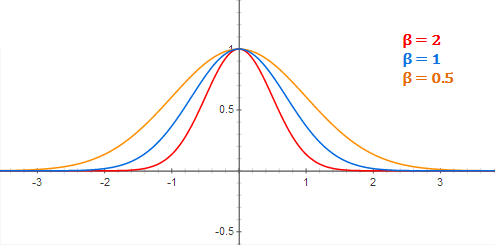
\includegraphics[width=\textwidth]{../figures/RBFactivation.png}
 \end{center}
\end{frame}

\begin{frame}
 \frametitle{Fonction à base radiale}
 \framesubtitle{Les couches d'un RBF}
 \incinslide{nnstruct.png}
\end{frame}

\subsection{Réseau de neurones récursif}
\begin{frame}
 \frametitle{Perceptron multi-couches récurrent}
 \framesubtitle{Un neurone récurrent d'un RMLP}
 \incinslide{neuronermlp.jpg}
\end{frame}

\begin{frame}
 \frametitle{Perceptron multi-couches récurrent}
 \framesubtitle{Les couches d'un RMLP}
 \begin{center}
  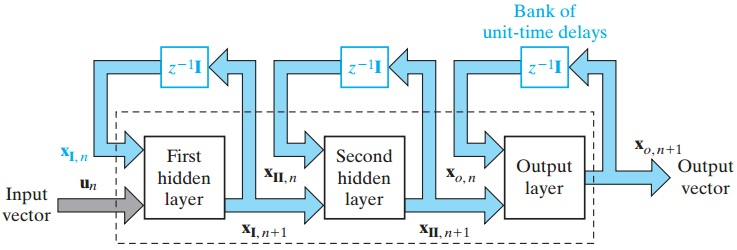
\includegraphics[width=\textwidth]{../figures/structurermlp.jpg}
 \end{center}
\end{frame}